%!TEX program = xelatex
\documentclass[dvipsnames, svgnames,a4paper,11pt]{article}
% ----------------------------------------------------
%   吉林大学通信工程学院信号与系统实验报告
%   原作者:Huanyu Shi,2019级
%     知乎:https://www.zhihu.com/people/za-ran-zhu-fu-liu-xing
%     Github:https://github.com/huanyushi/SYSU-SPA-Labreport-Template
%   在原基础上魔改了一些,更加贴近吉林大学实验格式。
% ----------------------------------------------------

% ----------------------------------------------------- 
%	加边框的命令
%	参考:https://tex.stackexchange.com/questions/531559/how-to-add-the-page-border-for-first-two-pages-in-latex
\usepackage{tikz}
\usetikzlibrary{calc}
\usepackage{eso-pic}
\AddToShipoutPictureBG{%
\begin{tikzpicture}[overlay,remember picture]
\draw[line width=0.6pt] % 边框粗细
    ($ (current page.north west) + (0.6cm,-0.6cm) $)
    rectangle
    ($ (current page.south east) + (-0.6cm,0.6cm) $); % 边框位置
\end{tikzpicture}}


\usepackage{xcolor}
\definecolor{c1}{HTML}{2752C9} % 目录颜色
\definecolor{c2}{RGB}{190,20,83} % 引用颜色

\usepackage{ctex}
\usepackage[top=28mm,bottom=28mm,left=15mm,right=15mm]{geometry}
\usepackage{hyperref} 
\hypersetup{
	colorlinks,
	linktoc = section, % 超链接位置,选项有section, page, all
	linkcolor = c1, % linkcolor 目录颜色
	citecolor = c1  % citecolor 引用颜色
}
\usepackage{amsmath,enumerate,multirow,float}
\usepackage{tabularx}
\usepackage{tabu}
\usepackage{subfig}
\usepackage{fancyhdr}
\usepackage{graphicx}
\usepackage{wrapfig}  
\usepackage{physics}
\usepackage{appendix}
\usepackage{amsfonts}

%
\usepackage{tcolorbox}
\tcbuselibrary{skins,breakable}
\newtcolorbox{tbox}[2][]{
    colframe=black!70!,
    breakable,
    enhanced,
	boxrule =0.5pt,
    title = {#2},
    fonttitle = \large\kaishu\bfseries,
	drop fuzzy shadow,
    #1
}
\newtcolorbox[auto counter,number within=section]{question}[1][]{
  top=2pt,bottom=2pt,arc=1mm,
  boxrule=0.5pt,
%   frame hidden,
  breakable,
  enhanced, %跨页后不会显示下边框
  coltitle=c1!80!gray,
  colframe=c1,
  colback=c1!3!white,
  drop fuzzy shadow,
  title={思考题~\thetcbcounter:\quad},
  fonttitle=\bfseries,
  attach title to upper,
  #1
}

% ---------------------------------------------------------------------
%	利用cleveref改变引用格式,\cref是引用命令
\usepackage{cleveref}
\crefformat{figure}{#2{\textcolor{c2}{图 #1}}#3} % 图片的引用格式
\crefformat{equation}{#2{(\textcolor{c2}{#1})}#3} % 公式的引用格式
\crefformat{table}{#2{\textcolor{c2}{表 #1}}#3} % 表格的引用格式


% ---------------------------------------------------------------------
%	页眉页脚设置
\fancypagestyle{plain}{\pagestyle{fancy}}
\pagestyle{fancy}
\lhead{\kaishu 吉林大学通信工程学院} % 左边页眉,学院 + 课程
\rhead{\kaishu 信号与系统实验报告} % 右边页眉,实验报告标题
\cfoot{\thepage} % 页脚,中间添加页码


% ---------------------------------------------------------------------
%	对目录、章节标题的设置
\renewcommand{\contentsname}{\centerline{\huge 目录}}
\usepackage{titlesec}
\usepackage{titletoc}
% \titleformat{章节}[形状]{格式}{标题序号}{序号与标题间距}{标题前命令}[标题后命令]
\titleformat{\section}{\centering\LARGE\songti}{}{1em}{}

% ---------------------------------------------------------------------
%   listing代码环境设置
\usepackage{listings}
\lstloadlanguages{python}
\lstdefinestyle{pythonstyle}{
backgroundcolor=\color{gray!5},
language=python,
frameround=tftt,
frame=shadowbox, 
keepspaces=true,
breaklines,
columns=spaceflexible,                   
basicstyle=\ttfamily\small, % 基本文本设置,字体为teletype,大小为scriptsize
keywordstyle=[1]\color{c1}\bfseries, 
keywordstyle=[2]\color{Red!70!black},   
stringstyle=\color{Purple},       
showstringspaces=false,
commentstyle=\ttfamily\scriptsize\color{green!40!black},%注释文本设置,字体为sf,大小为smaller
tabsize=2,
morekeywords={as},
morekeywords=[2]{np, plt, sp},
numbers=left, % 代码行数
numberstyle=\it\tiny\color{gray}, % 代码行数的数字字体设置
stepnumber=1,
rulesepcolor=\color{gray!30!white}
}




% ---------------------------------------------------------------------
%	其他设置
\def\degree{${}^{\circ}$} % 角度
\graphicspath{{./images/}} % 插入图片的相对路径
\allowdisplaybreaks[4]  %允许公式跨页


%---------------------------------------------------------------------------%
%->> User defined commands
%---------------------------------------------------------------------------%
\RequirePackage{mathrsfs}% script style math symbols % 导入模板的相关设置
\usepackage{lipsum}


%---------------------------------------------------------------------
%	正文
%---------------------------------------------------------------------

\begin{document}

\begin{table}
  \raggedleft
	\renewcommand\arraystretch{1.7}
	\begin{tabular}{|c|p{4em}|}
	\hline
	成绩 &  \\
	\hline
	教师签字 &   \\
	\hline
	\end{tabular}
\end{table}

\begin{center}
	{\kaishu \LARGE   \quad  \quad 通  \quad 信  \quad 工  \quad 程  \quad 学  \quad 院 }
  \newline
  \newline
  \newline
  \newline
  \newline
  {\kaishu \Huge 实 \quad  \quad  \quad 验  \quad  \quad  \quad 报 \quad  \quad  \quad 告}
  \newline
  \newline
  \newline
  \newline
  \newline
  {\songti \Huge  ( \quad  信  \quad 号  \quad 与  \quad 系  \quad 统 \quad)}
  \newline
  \newline
  \newline
  \newline
  \newline
  {\songti  \LARGE 实验题目:离散信号的频谱  \quad  \quad \quad}
\end{center}



\begin{table}[b]
	\renewcommand\arraystretch{1.7}
	\begin{tabularx}{\textwidth}{|X|X|X|X|}
	\hline
	专业:& 通信工程 &年级:& 2022级\\
	\hline
	姓名:& 苏睿杰  & 学号:& 20220826\\
	\hline
	实验时间:& 2023年11月3日 & 班级:& 42 \\
	\hline
	\end{tabularx}
\end{table}


%\clearpage
%\tableofcontents

\clearpage
\setcounter{section}{0}
\section{实验二十 \quad 离散信号的频谱}
	
\subsection*{一、实验目的}
\begin{enumerate}
	\item 观察离散信号并绘制其频谱,了解离散信号频谱的特点。
	\item 验证抽样定理。
\end{enumerate}

\subsection*{二、实验设备}
\begin{enumerate}
	\item 信号与系统试验箱。
	\item 数字信号发生器。
	\item 数字示波器。
	\item 选频电平表。
\end{enumerate}

\subsection*{三、实验原理}
\begin{enumerate}
  \item 离散时间信号可以从离散信号源获得,也可以从连续时间信号经抽样得到,抽样信号 $fs(t)$ 可以看成连续信号 $f(t)$ 和一组开关函数 $s(t)$ 的乘积,即 $fs(t)= f(t) s(t)$。
  
  \begin{figure}[htbp]
    \centering
    \subfloat[]{
      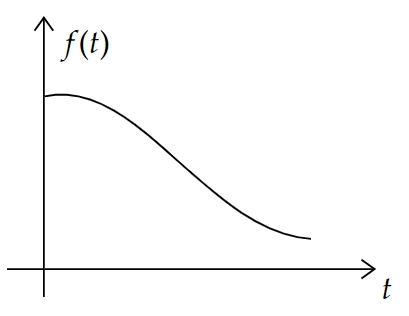
\includegraphics[width=0.3\textwidth]{1-a.png}
    }
    \subfloat[]{
      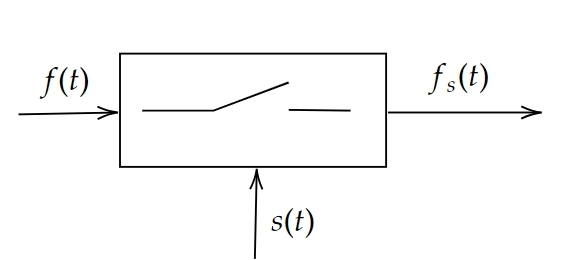
\includegraphics[width=0.3\textwidth]{1-b.png}
    }
    \subfloat[]{
      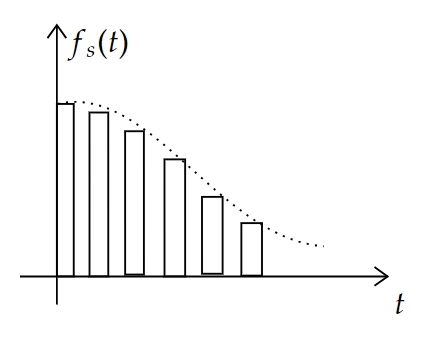
\includegraphics[width=0.3\textwidth]{1-c.png}
    }
    \caption{对连续时间信号进行取样}
  \end{figure}


  $s(t)$ 是一组周期性窄脉冲,周期 $T$ 称为抽样周期。其倒数 $f_s = \dfrac{1}{Ts}$称为抽样频率。
  
  若连续信号 $f(t)$ 的频谱如图2所示,则以 $f(t)$ 取样获得的取样信号 $f_s(t)$ 的频谱包括了原连续信号 $f(t)$ 的频谱以及无限个经过平移的原信号频谱,平移的频率间隔等于取样频率 $\omega_s = \dfrac{2\pi}{T_s}$,如图3所示,如果开关函数是周期性矩形脉冲,且脉冲宽度 $\tau$ 不为零时,则取信号 $f_s(t)$ 的频谱 $F_s(\omega)$ 的包络线按 $\dfrac{\sin x}{x}$ 的规律接减($X = \dfrac{n\pi \tau}{T_s}$)。
  
  取样信号 $f_s(t)$ 的频谱与连续时间信号测试方法一样,此时须注意频谱的周期性延拓。
  
  \begin{figure}[htbp]
    \centering
    \begin{minipage}[t]{0.48\textwidth}
    \centering
    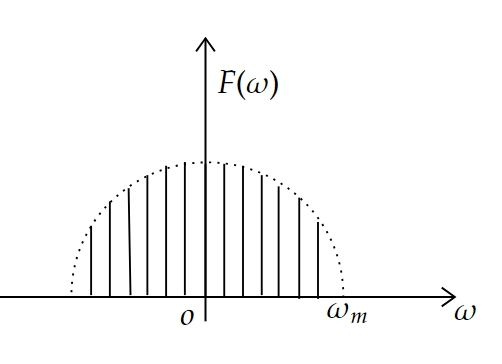
\includegraphics[width=6cm]{2.png}
    \caption{原信号频谱图}
    \end{minipage}
    \begin{minipage}[t]{0.48\textwidth}
    \centering
    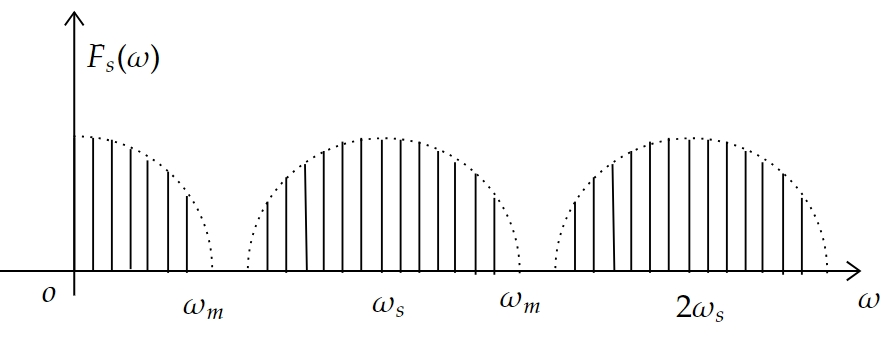
\includegraphics[width=9cm]{3.png}
    \caption{取样信号频谱}
    \end{minipage}
  \end{figure}
    


  \item 正如测得了足够的实验数据以后,我们可以在坐标纸上把一系统数据点连起来,得到一条光滑的曲线。抽样信号在一定条件下也可以恢复到原信号,只要用一截止频率等于原信号频谱中最高频率 $\omega_m$ 的低通滤波器滤除高频分量,而仅存原信号频谱的频率成分,这样,低通滤波器的输出是得到恢复的原信号。
  
  根据采样定理,原信号得以恢复的条件是取样频率 $f_s \ge 2B$。$f_s$ 为取样频率,$B$ 为原信号的有效频带宽度。当取样频率 $f_s < 2B$ 时,取样信号的频谱会发生混迭。如图4所示,此时,我们无法用低通滤波器获得原信号频谱的全部信息内容。
  
  \begin{figure}[htbp]
    \centering
    \subfloat[]{
      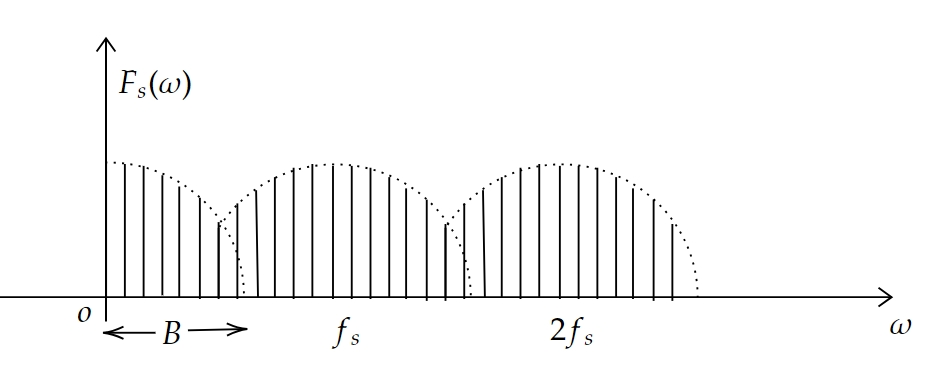
\includegraphics[width=0.8\textwidth]{4.png}
    }
    \caption{$f_s < 2B$ 时,取样信号频谱}
  \end{figure}

  实验中选用 $f_s<2B$,$f_s=2B$,$f_s > 2B$ 三种抽样频率对连续信号进行抽样,以验证抽样定理一要使信号抽样后能不失真地还原,抽样频率 $f_s$ 必须大于信号频谱中最高频率的两倍。

  \item 有效频带宽度:严格地说,周期性信号所包含的谐波分量有无限多,不过由于谐波振幅随频率增高而减小,通常只考虑频率较低的一些分量就够了。从 $0$ 频率到需要考虑最高次谐波频率间的频段称为信号的频带宽度。信号频带宽度的具体定义视情况而定,有时将谐波振幅下降到最大值的 $\dfrac{1}{K}$(例如 $\dfrac{1}{10}$)的频段称为信号的频带宽度。本实验对于周期正弦信号频率为 $25KHz$,从频谱图可以看出,该信号为单频信号,抽样脉冲控制信号频率 $f_s$ 取 $5OKHz$。对于周期方波和三角波信号,若其基频率为 $5KHz$,从频谱图可以看出,可取 $5$ 倍于基波频率作为有效的频带宽度,则抽样脉冲控制信号的频率 $f_s$ 取 $50KHz$。
  
  \item 理论计算:在理论情况下,对于给定的方波 $f(t)$(频率为 $5kHz$)以及周期矩形脉冲 $s(t)$(频率为 $100kHz$),可以计算出 $f(t)$ 和 $s(t)$ 的幅度谱函数,对于取样信号 $f_s(t) = f(t)s(t)$,同样可以计算出 $f_s(t)$ 的幅度谱函数(太过复杂,较难算出,在这里不列出来了),下式是自己计算的 $F(j\omega)$ 和 $S(j\omega)$ 的理论结果。
    \begin{equation}
      F(j\omega) = \sum_{n = 1}^{\infty}\dfrac{2}{jn}[1 - (-1)^n][\delta(\omega - n\dfrac{2\pi}{T}) - \delta(\omega + n\dfrac{2\pi}{T})]
    \end{equation}
    \begin{equation}
      S(j\omega) = \sum_{-\infty}^{+\infty}\dfrac{1}{nj}[1 - e^{-jn\frac{2\pi}{T}\tau}] \delta(\omega - n\dfrac{2\pi}{T})
    \end{equation}
    \begin{equation}
      \mathscr{F}[f_s(t)] = \dfrac{1}{2\pi}F(j\omega) * S(j\omega)
    \end{equation}
  \begin{figure}[htbp]
    \centering
    \subfloat[]{
      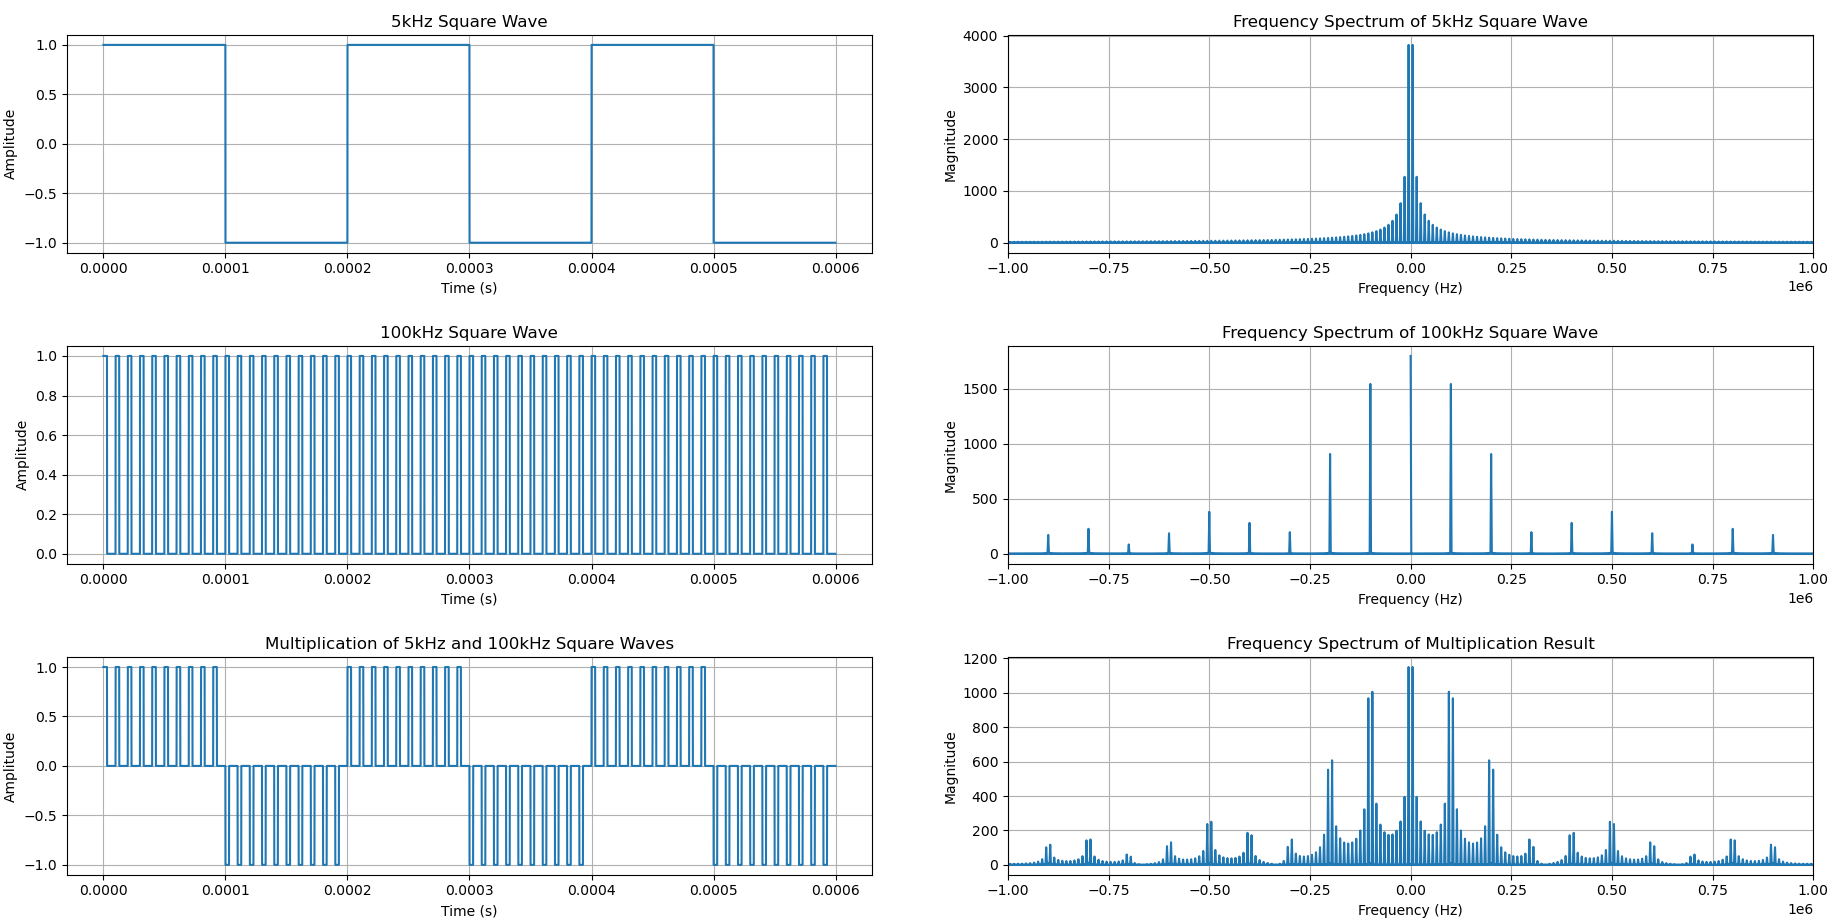
\includegraphics[width=1.0\textwidth]{11.png}
    }
    \caption{$f(t), s(t), f_s(t)$ 的波形图以及幅度谱}
  \end{figure}
\end{enumerate}

\subsection*{四、实验注意事项}
\begin{enumerate}
  \item 只有当取样脉冲的频率与被取样信号1频率保持整数倍数关系时,示波器上才能得到稳定的波形,故需微调脉冲的频率。
  \item 被取样信号的幅度不宜过大。否则将得不到良好的离散信号。
\end{enumerate}

\subsection*{五、实验内容与步骤}
\begin{enumerate}
  \item 输入信号为 $5KHz$ 的方波信号,$V_{p-p} = 2V$,观察抽样后离散方波信号的波形并测绘出其频谱图。
  \begin{enumerate}
    \item[(1)] 用选频电平表测量抽样后离散信号 $f_s(t)$ 的频谱。 
    \begin{table}[htbp]
      \renewcommand\arraystretch{1.7}
      \centering
      \caption{}
      \begin{tabularx}{\textwidth}{|p{0.06\textwidth}|X|X|X|X|X|X|X|X|X|X|X|X|X|X|X|}
        \hline
        f(kHz) & 5 & 15 & 25 & 35 & 45 & 55 & 65 & 75 & 85 & 95 & 105 & 115 & 125 & 135 & 145 \\
        \hline
        Pn(dB) & \tiny{-7.4}	& \tiny{-17.5}	& \tiny{-23}	& \tiny{-26.7}	& \tiny{-30.4}	& \tiny{-31.1}	& \tiny{-30.4}	& \tiny{-25.5}	& \tiny{-20.6}	& \tiny{-10.6}	& \tiny{-10.6}	& \tiny{-20.6}	& \tiny{-25.7}	& \tiny{-31}	& \tiny{-33.8}
        \\
        \hline
        Un & 0.33 & 0.10 & 0.05	& 0.04 & 0.02	& 0.02 & 0.02 & 0.04 & 0.07	& 0.23 & 0.23	& 0.072	& 0.04 & 0.02	& 0.02
        \\
        \hline
      \end{tabularx}
    \end{table}
    
    注:$U_n = 0.775 \times 10^{\frac{P_n}{20}}$

    \item[(2)] 调整 $f(t)$ 和 $s(t)$ 的频率,使抽样信号通过滤波器后能较好地复原。
    \item[(3)] 改变抽样频率为 $f_s < 2B$ 和 $f_s \ge 2B$,观察并描绘复原后的信号,比较其失真程度。
  \end{enumerate}
  \item 根据实验所得数据作出了频谱图,如下图所示:
    \begin{figure}[htbp]
      \centering
      \subfloat[]{
        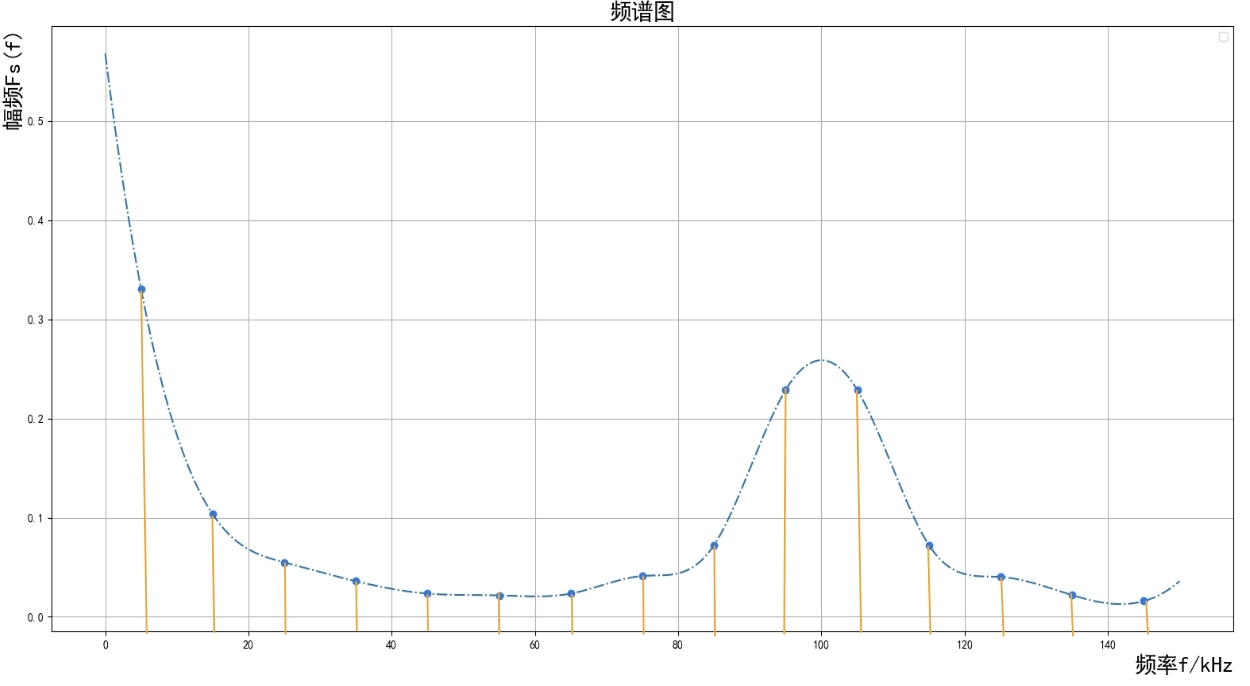
\includegraphics[width=0.8\textwidth]{6.png}
      }
      \caption{抽样后离散信号 $f_s(t)$ 的频谱}
    \end{figure}
  \item 分别改变抽样频率 $f_s$,并观察复原后信号的失真程度。
    
    根据信号频带宽度的定义,一般取谐波下降到最大值的 $\dfrac{1}{10}$ 左右的频段作为带宽。对于方波,$n$ 取不到 $10$,故令 $n = 9$,对应 $B = 5 \times 9 = 45kHz$。

    根据抽样定理,要使抽样信号无失真的还原,须使抽样频率以最高频率的两倍为临界点,故将 $2B = 90kHz$ 作为是否失真的临界状态。
    
    故接下来的实验会分别让 $f_s < 2B$,$f_s = 2B$,$f_s > 2B$ 来进行实验。
    \begin{enumerate}
      \item $f_s < 2B$,此时 $f_s = 60 kHz$,如图7所示。
        \begin{figure}[htbp]
          \centering
          \subfloat[]{
            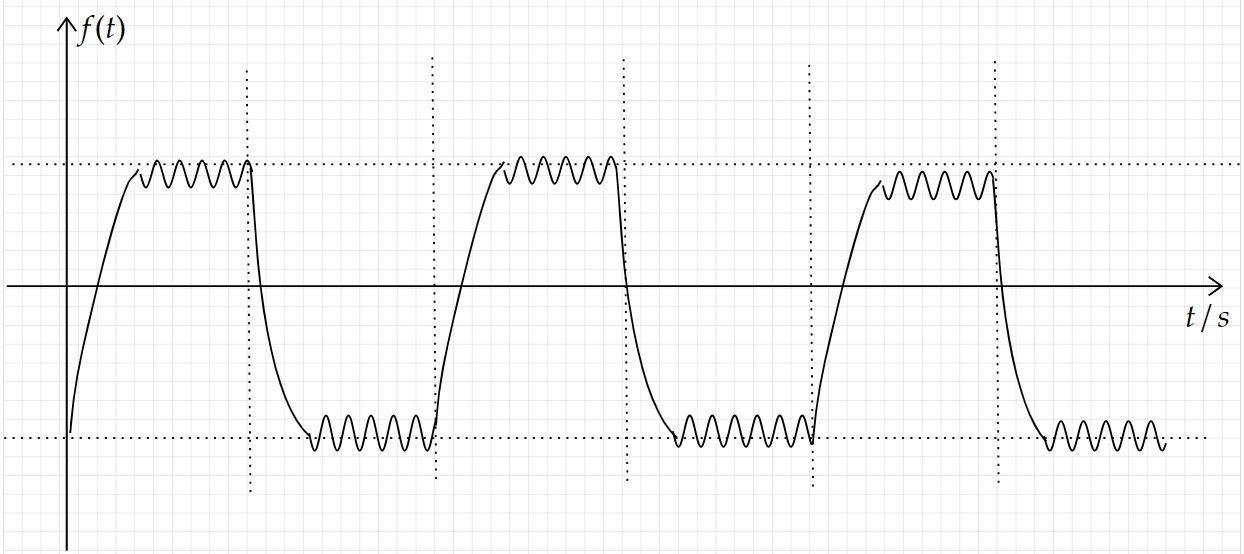
\includegraphics[width=0.8\textwidth]{9.png}
          }
          \caption{抽样频率 $f_s < 2B$ 的复原信号}
        \end{figure}
      \item $f_s = 2B$,此时 $f_s = 90 kHz$,如图8所示。
        \begin{figure}[htbp]
          \centering
          \subfloat[]{
            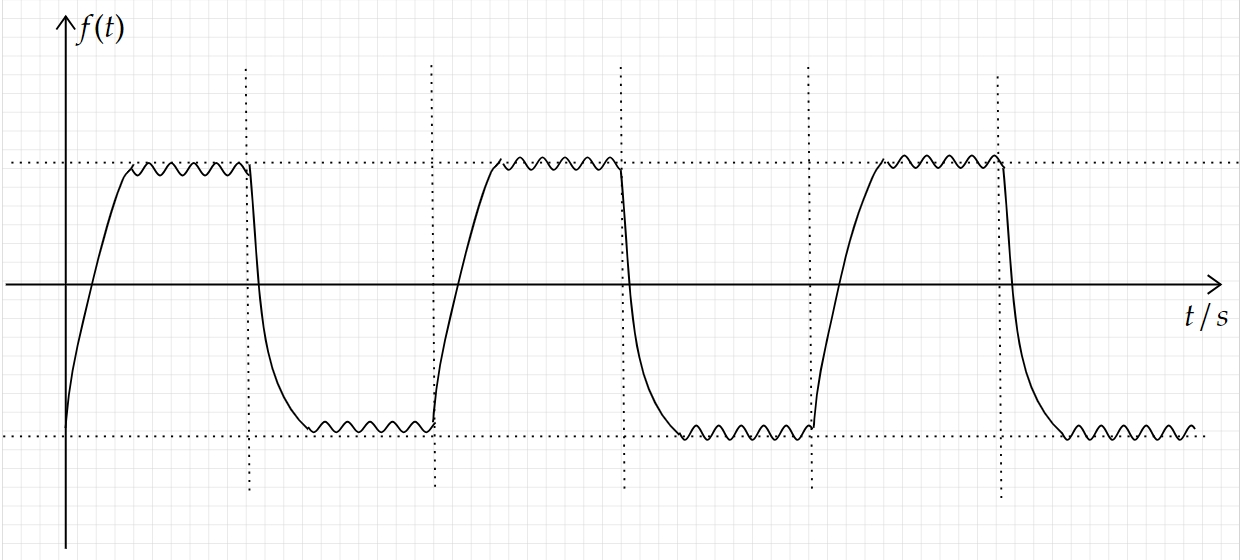
\includegraphics[width=0.8\textwidth]{8.png}
          }
          \caption{抽样频率 $f_s > 2B$ 的复原信号}
        \end{figure}
      \newpage
      \item $f_s > 2B$,此时 $f_s = 130 kHz$,如图9所示。
        \begin{figure}[htbp]
          \centering
          \subfloat[]{
            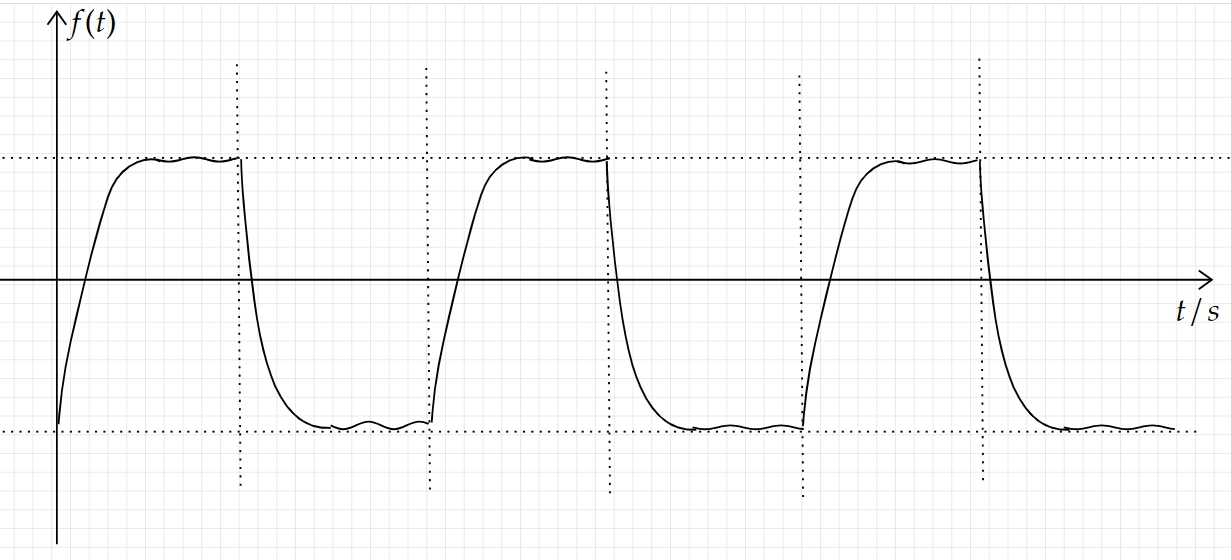
\includegraphics[width=0.8\textwidth]{7.png}
          }
          \caption{抽样频率 $f_s > 2B$ 的复原信号}
        \end{figure}
    \end{enumerate}
\end{enumerate}

\subsection*{六、误差分析}
\begin{enumerate}
  \item 由于实验仪器参数和理论值有所误差,故所得数据可能会和理论不同。
  \item 在使用电平表读数时,肉眼观察可能存在一定误差,会与理论有一定偏差。
\end{enumerate}

\subsection*{七、实验结论及总结}
\begin{enumerate}
  \item $f_s(t)$ 的频谱图随频率增大振幅逐渐减小,与理论情况大致相等。
  \item 当抽样频率 $f_s < 2B$ 时,此时复原后的函数失真较为严重,所得图像与 $f(t)$ 之间的误差较大。
  \item 当抽样频率 $f_s = 2B$ 时,此时复原后的函数有一定失真,但比 $f_s < 2B$ 时要好很多,所得图像已经较为接近 $f(t)$。
  \item 当抽样频率 $f_s > 2B$ 时,此时复原后的函数几乎没有失真,所等图像与 $f(t)$ 最为接近,复原程度最好,最接近方波。
\end{enumerate}

\end{document}
